\chapter{Sucesiones}

\begin{tikzpicture}
	\fill [left color=red!50, right color=teal!50] (0,0) rectangle (6.5,.2);
	\fill [left color=teal!50, right color=blue!50] (6.5,0) rectangle (11.5,.2);
	\end{tikzpicture}


\vspace{15mm}


\begin{adjustwidth}{40pt}{40pt}
\begin{cuadro-gris}

	\begin{multicols}{2}
	$\triangleright \quad$  Sucesiones. Término general.
	
	$\triangleright \quad$  Progresiones aritméticas y geométricas.
	
	$\triangleright \quad$  Monotonía y acotación.
	
	$\triangleright \quad$  Aproximación al concepto de límite de una sucesión.
	\end{multicols}
	
\end{cuadro-gris}
\end{adjustwidth}



\vspace{5mm}
\section{Sucesión. Término general}

\begin{tikzpicture}
	\fill [left color=red!50, right color=teal!50] (0,0) rectangle (3.5,.1);
	\fill [left color=teal!50, right color=blue!50] (3.5,0) rectangle (7.5,.1);
	\end{tikzpicture}
\vspace{0.5cm}

\begin{definition}[ Sucesión.]

Una sucesión es un conjunto ordenado de números reales :
                        $\  a_1, a_2, a_3, a_4, a_5, \cdots \equiv \{a_n\}$
                         
                         
\vspace{2mm} Se trata de funciones reales de variable natural: $\{a_n\}:\ \mathbb N \longrightarrow \mathbb R\, , $ la variable independiente es un número natural y la variable dependiente es un número real. 
                         
                         
\vspace{2mm} Las sucesiones se suelen representar por letras latinas minúsculas con el subíndice $n$ y encerradas entre llaves, $\{a_n\}$. A cada uno de los números que  la forman  se les llama \emph{término} de la sucesión y se designa por $a_i$, siendo  $i$  la posición o lugar dicho término ocupa  en la sucesión.
\end{definition}

\begin{miejemplo}


\begin{table}[H]
%\centering
\begin{tabular}{llll}
 & $\{a_n\}	\, :\ 1,3,5,7,9, \cdots$ &  & $\to \ a_3=\ 5$ \\
 & $\{b_n\}	\, :\ 2,4,8,16,32, \cdots$ &  & $\to \ b_5=32$ \\
 & $\{c_n\}	\, :\ 1,4,27,256, \cdots$ &  & $\to \ c_2=\ 4 $
\end{tabular}
\end{table}
\end{miejemplo}

\begin{definition}[ Término general.]

El término general de una sucesión es una expresión (fórmula) que nos permite calcular cualquier término de la sucesión sabiendo el lugar que ocupa, lo representamos por $a_n$.	

\vspace{2mm} Su utilidad es doble:

--- Permite calcular cualquier término de la sucesión sin más que saber el lugar que éste ocupa. Es por ello que el término general representa a toda la sucesión.

--- También es útil para averiguar si un numero dado es o no un término de la sucesión y, si lo es, averiguar la posición que ocupa.
\end{definition}

\begin{miejercicio}

Considerar la sucesión cuyo término general está definido por  $a_n=\dfrac{3n+2}{2n-1}	$

\begin{enumerate}[a) ]
\vspace{-2mm} \item Calcula los tres primeros términos y el undécimo.
\vspace{-3mm} \item Averigua si el número $53/33$ es o no un término de la sucesión.
\vspace{-3mm} \item Haz lo mismo para el número $26/25$
\end{enumerate}

\vspace{-4mm}
\rule{250pt}{0.1pt}
\vspace{5mm}

$\triangleright \ a)\qquad a_1=\dfrac{3(1)+2}{2(1)-1}=5;\ \ a_2=\dfrac{3(2)+2}{2(2)-1}=\dfrac 8 3 ;\ \ a_3=\dfrac{3(3)+2}{2(3)-1}=\dfrac{11}{5};\ \ a_11=\dfrac 5 3$

\vspace{2mm}$\triangleright \ b)\qquad \dfrac{3n+2}{2n-1}=\dfrac {53}{33} \to 99n+66=106n-53 \to 119=7n \to n=\dfrac{119}{7}=17 \in \mathbb N $

\vspace{2mm}Sí, efectivamente ${53}/{33}$ es un término de la sucesión $\{a_n\}$ (o, abusando del lenguaje, de la sucesión $a_n$). Además, se trata del término decimoséptimo, así, $a_{17}=55/33$

\vspace{2mm}$\triangleright \ c)\qquad \dfrac{3n+2}{2n-1}=\dfrac{26}{25} \to 75n+50=52n-26 \to 23n=24 \to n=\dfrac{24}{23} \notin \mathbb N$

\vspace{2mm}No, el número $26/25$ no es un término de la sucesión $a_n \, , \ (26/25 \notin a_n)$.

\end{miejercicio}

Decimos que una sucesión es \textbf{recurrente} o está definida por \emph{recurrencia} cuando cada término, a partir de uno dado, se obtiene en función de dos o más de sus  anteriores. En estos casos no siempre es sencillo encontrar el término general; p. e.: $\ \{a_n\}:\ \ 1, 2, 3, 0, 5, -2, 7, \cdots$

$\textcolor{gris}{a_1=1,\ a_2=2,\ a_3=3,\ a_n=a_{n-3}+a_{n-2}-a_{n-1};\ \forall n>3}$.

\vspace{5mm}
\begin{myexampleblock}{La sucesión de Fibonacci}

\vspace{2mm} \emph{Supongamos que un par de conejos recién nacidos, un macho y una hembra se colocan en el campo. Los conejos son fértiles a la edad de un mes, así que al final del segundo mes una hembra puede producir otro par de conejos. Supongamos que nuestros conejos nunca mueren, y que las hembras siempre producen un nuevo par (un macho y una hembra) cada mes, desde el segundo mes de vida. La pregunta que Fibonacci se hizo fue la siguiente, ?`cuántos pares de conejos tendremos en un año?}

\vspace{4mm} \small{\textsf{Este es el famoso problema de los conejos que Leonardo de Pisa (1170-1241), conocido como Fibonacci, plantea (entre otros problemas) en su libro “Liber Abaci” (1202).}}

\begin{figure}[H]
	\centering
	\includegraphics[width=0.9\textwidth]{img-suc/suc01.png}
	\caption*{\scriptsize{imagen : $\ $ https://oscarenfotos.com/2019/04/06/proporcion-aurea-y-fotografia/conejos\_fibonacci/}}
	\end{figure}
 
\vspace{2mm} Si observamos atentamente del enunciado del problema deducimos que:
\vspace{-1mm}
\begin{itemize}
	
\vspace{-2mm}\item Al final del primer mes, hay un solo par.

\vspace{-2mm}\item Al final del segundo mes, la hembra produce un nuevo par, así que ahora
tenemos dos parejas de conejos en el campo.

\vspace{-2mm}\item Al final del tercer mes, la hembra inicial produce un segundo par, haciendo que
en el campo tengamos tres pares de conejos.

\vspace{-2mm}\item Al final del cuarto mes, la hembra original ha producido otro nuevo par y la
hembra nacida dos meses antes produce su primer par, con lo que tendremos 5 pares.
\end{itemize}

\vspace{2mm} El número de pares de conejos en el campo al inicio de cada mes es:
$1, 1, 2, 3, 5, 8, 13, 21, 34, 55, 89, 144, \cdots$,
una sucesión, que se inicia con $1$ y $1$ donde cada nuevo término es la suma de los dos anteriores, y que recibe el nombre de \emph{sucesión de Fibonacci}: $\ \ \boldsymbol{ a_1=a_2=1;\ \ a_n=a_{n-1}+a_{n-2}\, , \ \forall n>2 }  \ \ (n\in \mathbb N)$ 

\vspace{2mm} Si hacemos el cociente de dos números consecutivos de la sucesión obtenemos esta otra:
$1/1=1, 2/1=2, 3/2=1.5, 5/3=1.666, 8/5=1.6, 13/8=1.625, 21/13=1.61538, \cdots$

\vspace{2mm} El cociente entre dos términos consecutivos de la sucesión tiende a un valor particular, el cual recibe el nombre de \emph{número de oro} o \emph{divina proporción} y tiene un valor aproximado de 1.61804, se representa por la letra griega phi, $\phi=\frac{1+\sqrt{5}}{2}$. 

\vspace{2mm}  La sucesión de Fibonacci tiene numerosas aplicaciones en ciencias de la computación, matemática y teoría de juegos. También aparece en configuraciones biológicas, como por ejemplo en las ramas de los árboles, en la disposición de las hojas en el tallo, en las flores de alcachofas y girasoles, en las inflorescencias del brécol romanesco, en la configuración de las piñas de las coníferas y en cómo el ADN codifica el crecimiento de formas orgánicas complejas. De igual manera, se encuentra en la estructura espiral del caparazón de algunos moluscos, como el nautilus.


\vspace{4mm} 
\begin{footnotesize}
Se puede encontrar su término general: $\ \ a_n=\dfrac 1{\sqrt{5}} \left[ \left(\dfrac{1+\sqrt{5}}{2}\right)^n-\left(\dfrac{1-\sqrt{5}}{2}\right)^n \right] =\dfrac{\phi^n-\phi^{-n}}{\sqrt{5}}=f_n$
\end{footnotesize}
\end{myexampleblock}


\begin{miejercicio}
. \normalsize{Determina} los cinco primeros términos de las sucesiones cuyos términos generales son:

\begin{multicols}{2}
$a_n=(-3)^n$

$b_n=3^{-n}$

$c_n=3n+1$

$d_n=\dfrac{n^2+1}{n^2}$

$e_n=n!-(n-1)!$

$\quad$

$\begin{cases} g_1=5 \\ g_2=-1\end{cases} \ \ g_n=g_{n-1}+2g_{n-
2},\, \forall n>2$	
\end{multicols}

\rule{250pt}{0.1pt}

\begin{multicols}{2}
\vspace{2mm} $\triangleright \ \ \{a_n\}:\ -3,\, 9,\, -27,\, 81,\, -243$

\vspace{2mm} $\triangleright \ \ \{b_n\}:\ 1/3,\ 1/9,\ 1/27,\ 1/81,\ 1/243$

\vspace{2mm} $\triangleright \ \ \{c_n\}:\ 4,\, 7,\, 10,\, 13,\, 16$

\vspace{2mm} $\triangleright \ \ \{d_n\}:\ 2,\, 5/4,\, 10/9,\, 17/16,\ 26/25$

\vspace{2mm} $\triangleright \ \ \{e_n\}:\ 0,\, 1,\ 4,\, 18,\, 96$

\vspace{2mm} $\triangleright \ \ \{g_n\}:\ 5,\, -1,\, 9,\, 7,\, 25$
\end{multicols}
	
\end{miejercicio}


\begin{miejercicio}

Encuentra, a ojo, el término general de las sucesiones cuyos primeros términos son:

\begin{multicols}{2}
	\vspace{2mm} $\triangleright \ \ \{a_n\}:\ 10,\, 20,\, 30,\, 40,\, \cdots$

\vspace{2mm} $\triangleright \ \ \{b_n\}:\ 2,\ 4,\ 6,\ 8,\ \cdots$

\vspace{2mm} $\triangleright \ \ \{c_n\}:\ 1,\, 3,\, 5,\, 7,\, \cdots$

\vspace{2mm} $\triangleright \ \ \{d_n\}:\ -1,\, 1,\, -1,\, 1,\ \cdots$

\vspace{2mm} $\triangleright \ \ \{e_n\}:\ 1,\, -4,\ 9,\, -16,\, \cdots$

\vspace{2mm} $\triangleright \ \ \{g_n\}:\ 7,\,7,\, 7,\, 7,\, \cdots$
\end{multicols}


\rule{250pt}{0.1pt}

\begin{multicols}{3}

\vspace{2mm}  $a_n=10n$

\vspace{2mm}  $b_n=2n$

\vspace{2mm}  $c_n=2n-1$

\vspace{2mm}  $d_n=(-1)^n$

\vspace{2mm}  $e_n=(-1)^{n+1} \ n^2$

\vspace{2mm}  $g_n=7$
	
\end{multicols}

\end{miejercicio}


\vspace{1cm}
\section{Progresiones aritméticas}

\begin{tikzpicture}
	\fill [left color=red!50, right color=teal!50] (0,0) rectangle (3.5,.1);
	\fill [left color=teal!50, right color=blue!50] (3.5,0) rectangle (7.5,.1);
	\end{tikzpicture}
\vspace{0.5cm}


\begin{definition}[ Progresión aritmética: PA]

Una progresión aritmética (PA) es una sucesión en la que cada término, salvo el primero, se obtiene sumando una cantidad constante al término anterior. Esta cantidad se llama \emph{distancia} o  diferencia de la progresión y se representa por $d$. Es por ello que si $\{a_n\}$ es una PA entonces queda unívocamente determinada al conocer $a_1$ y $d$.
\end{definition}


\vspace{4mm} Búsqueda del término general de una PA:
\begin{table}[H]
\centering
\begin{tabular}{ccccccccccc}
$a_1$ &  & $a_2$ &  & $a_3$ &  & $a_4$ & &$\cdots$ &  & $a_n$ \\
 & $+d$ &  & $+d$ &  & $+d$ & & $+d$ &  & $\cdots$ &   \\
$a_1$ &  & $a_1+d$ &  & $a_1+2d$ &  & $a_1+3d$ &  &$\cdots$ & & $a_1+(n-1)d$
\end{tabular}
\end{table}

\begin{definition}[ Término general de una PA]
. El término general de una progresión aritmética es :

$$\boxed{ \ 	\boldsymbol{ a_n  \ =  \  a_1 \, + \,   ( n - 1 )  \cdot  d } \ }$$
\end{definition}



\begin{miejercicio}

Encuentra el término general de las sucesiones cuyos primeros términos son:

$\{a_n\}:\ 13,15,17,19,\cdots \qquad  \qquad \{b_n\}:\ 11,7,3,-1,\cdots$

\rule{250pt}{0.1pt}
\vspace{2mm}
	
En la primera sucesión, cada término se obtiene del anterior al sumarle $d=2$ (las diferencias entre términos consecutivos es constante), se trata de un PA. Como el primer término es $a_1=13$, tenemos una $PA\begin{cases} \ a_1=13 \\ \ d=2 \end{cases}$.

\vspace{2mm} Su término general es:
$\quad a_n=13+(n-1)\cdot 2 \ \to \ \boldsymbol{a_n=2n+11}$

\vspace{4mm}

En la segunda sucesión, cada término se obtiene del anterior al sumarle $d=-4$ (las diferencias entre términos consecutivos es constante), se trata de un PA. Como el primer término es $b_1=11$, tenemos una $PA\begin{cases} \ b_1=11 \\ \ d=-4 \end{cases}$.

\vspace{2mm} Su término general es:
$\quad b_n=11+(n-1)\cdot (-4) \ \to \ \boldsymbol{b_n=-4n+15}$


\end{miejercicio}


\vspace{10mm}
\subsection{Suma de términos consecutivos de una progresión aritmética}
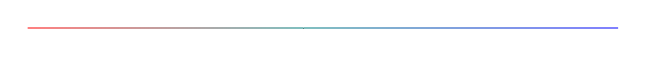
\begin{tikzpicture}
	\fill [left color=red!50, right color=teal!50] (0,0) rectangle (3.5,.01);
	\fill [left color=teal!50, right color=blue!50] (3.5,0) rectangle (7.5,.01);
	\end{tikzpicture}
\vspace{0.5cm}

\begin{large}\textbf{Interpolación de términos en una PA}\end{large}

\normalsize{Interpolar} $m$ medios aritméticos entre otros dos $a<b$ es encontrar una PA de $m+2$ términos de modo que $a, \, a_1,\ \cdots,\, a_m,\, b$ sea una PA. La distancia entre términos será (decimos que son medios porque están entre otros dos y aritméticos por tratarse de progresiones aritméticas):

$a_n=a_1+(n-1)d \ \to a_{m+2}=\boldsymbol b=a_1+[(m+2)-1] d= \boldsymbol{a+(m+1)d} \ \to \ \  \boldsymbol{ d=\dfrac{b-2}{m+1} }$

\vspace{5mm}\begin{large}\textbf{Suma de términos equidistantes en una PA}\end{large}

Los términos que equidistan de los extremos de una PA suman lo mismo que estos: 

$\text{Si } a_i,\, a_j \ \text{ son equidistantes en PA } \ \Rightarrow \ a_i+a_j=a_1+a_n$ 

\underline{Demostración}:

Los subíndices de los términos equidistantes han de ser tal que $i+j=n+1 \ \to j=n+1-i$

$a_i+a_j=a_i+a_{n+1-i}=a_1+(i-1)d+a_1+(n+1-i-1)d=a_1+(i-1)d+a_1+(n-i)d=2a_1+(i-1+n-i)d=2a_1+(n-1)d=a_1+a_1+(n-1)d=a_1+a_n$ \QED


\begin{myexampleblock}{Anécdota de Gauss}
\begin{multicols}{2}
\emph{``J. B. Büttner, maestro de un colegio alemán, castigó a todos los niños a sumar los 100 primeros números naturales para tenerlos entretenidos y callados un buen rato. Uno de los niños, Carl Friedrich Gauss obtuvo la respuesta casi de inmediato:  1 + 2 + 3 + … + 99 + 100  = 5050 .''}

\vspace{2mm} \emph{?`Cómo lo hizo?. Pues se dio cuenta de que la suma del primer número con el último (1+100) era igual que la del segundo número y el penúltimo (2+99), y así sucesivamente. Por lo que, como había cien números, se formaban 50 parejas con la misma suma, es decir 101. Por lo que sólo faltaba multiplicar 101 x 50 = 5.050.}

\begin{figure}[H]
	\centering
\includegraphics[width=0.4\textwidth]{img-suc/suc08.png}
	\end{figure}
\end{multicols}

\begin{small} \textsf{Johann Carl Friedrich Gauss (1777-1855) fue un niño prodigio que nació en una familia humilde y de padres analfabetos pero que fue autodidacta para aprender a leer y llegar a ser conocido como ``el príncipe de los matemáticos'' y reconocido por sus coetáneos como el ``matemático más grande desde la antigüedad''}.\end{small}
\end{myexampleblock}




\vspace{5mm}\begin{large}\textbf{Suma de los  $\boldsymbol n$  primeros términos de una PA}\end{large}

\vspace{3mm}
\begin{theorem}

La suma de $n$ términos consecutivos de una PA es igual a la semisuma de los extremos multiplicado por el número de términos.

$$\{a_n\}:\ PA \qquad a_1+a_2+a_3+\cdots + a_{n-1}+a_n= \displaystyle \sum_{k=1}^n	a_k = \ \boxed{ \boldsymbol{S_n\ = \ \ \dfrac{a_1+a_n}{2}\cdot n} \ }$$
\end{theorem}

\underline{Demostración}:

Disponiendo de derecha a izquierda la suma de términos y colocando debajo la misma en orden inverso y sumando, se observa que, en vertical, aparece $n$ veces la suma términos equidistantes, por la propiedad anterior, la suma de los extremos.

\begin{table}[H]
%\scriptsize
\centering
\begin{tabular}{c|cccccc}
$S_n \quad $ & $a_1$ & $a_2$ & $a_3$ & $\quad  \cdots \quad $ & $a_{n-1}$ & $a_n$ \\
$S_n \quad  $ & $a_n$ & $a_{n-1}$ & $a_{n-2}$ & $\cdots$ & $a_2$ & $a_1$ \\ \hline
$2\, S_n$ & $\quad a_1+a_n \quad $ & $a_2+a_{n-1}$ & $a_3+a_{n-2}$ & $\cdots$ & $a_{n-1}+a_2$ & $a_n+a_1$ \\ \hline
$2\, S_n$ & $\quad a_1+a_n \quad $ & $a_1+a_n$ & $a_1+a_n$ & $\cdots$ & $a_1+a_n$ & $a_1+a_n$
\end{tabular}
\end{table}

Luego $\quad 2S_n = n\, (a_1+a_n) \ \to \ \ S_n\ = \ \ \dfrac{a_1+a_n}{2}\cdot n$\QED

\vspace{5mm}

\begin{miejercicio}

Interpola tres términos aritméticos entre -12 y 8.

\rule{250pt}{0.1pt}
\vspace{2mm}

$a=-12;\ b=8;\ m=3 \quad \to \quad d=\dfrac{8-(-12)}{3+1}=\dfrac{20}{4}=5$

\vspace{2mm} Los términos buscados son: $\quad -2;\ \boldsymbol{-7, \ -2, \ 3}  ; \ 8$	

\vspace{2mm}\begin{small} \textcolor{gris}{De otro modo: $-12,x,y,z,8:\ PA \to 8=-12+(5-1)d \to d= 5:\ \  -2;\ \boldsymbol{-7, \ -2, \ 3}  ; \ 8 $} \end{small}
\end{miejercicio}

\begin{miejercicio}

\normalsize{Calcula} la suma de los 100 primeros números naturales:
$1+2+3+\cdots +99+100=?$
\rule{250pt}{0.1pt}	

Tenemos una PA cuyo primer término es $1$, el último $100$ (hay $100$ términos) y cuya distancia es $1$. Nos preguntan por la suma de todos ellos.

\vspace{2mm} $S_{100} =\  \textcolor{gris}{S_n=\dfrac{a_1+a_n}{2}\, n} \ = \dfrac{1+100}{2}\, 100= 50.5\cdot 100=\ 5050 \quad $ \textcolor{gris}{(Problema de Gauss)}
\end{miejercicio}


\begin{miejercicio}

Calcula la suma de todos los múltiplos de $7$ comprendidos entre $250$ y $500$.

\rule{250pt}{0.1pt}
\vspace{2mm}

Los múltiplos de siete, $\dot{7}$, son números de la forma $7k,\ \forall k\in \mathbb N$. Forman una PA ya que pasa pasar de un múltiplo de $7$ al siguiente hay que sumarle $7:\ \ a_n=a_1+(n-1)\, 7$

\vspace{2mm}--- Búsqueda del primer término: $\ 7k=250 \to k=35.71\cdots \to 7\cdot 35=245 \to 245+7=\boldsymbol{252=a_1}\ $ Primer $\dot{7}$ en $[250,500]$.

\vspace{2mm}--- Búsqueda del último término: $\ 7k=500 \to k=71.42\cdot \to 7\cdot 71=\boldsymbol{497=a_n}\ $ Último $\dot{7}$ en $[250,500]$.

\vspace{2mm}--- Búsqueda del número de términos: $\ PA:\ a_1=252;\ d=7 \ \to a_n=a_1+(n-1)d\, : \ a_n=497=252+7(n-1) \to n-1=\dfrac{497-252}{7}=35 \to \boldsymbol{n=36}\ $ Hay un total de $36$ términos $\dot{7}$ en $[250,500]$. 

\vspace{2mm}Tenemos que sumar los $n=36$ términos de una PA en que $a_1=252$ y $a_n=497$, aplicando la fórmula:

\vspace{2mm} $S_{36} =\  \textcolor{gris}{S_n=\dfrac{a_1+a_n}{2}\, n} \ = \dfrac{252+497}{2}\, 36= \ 13482$

\end{miejercicio}


\vspace{5mm}

\begin{myalertblock}{Progresiones aritméticas de segundo orden}

\vspace{2mm} Una \emph{progresión aritmética de segundo orden} es una sucesión cuyo término general es un polinomio de segundo grado en $n:\quad a_n=An^2+Bn+C\, , \ n\in \mathbb N;\ \ A,B,C \, \text{constantes}$.
	
\vspace{2mm} La diferencia entre términos consecutivos no es ahora constante, es una PA (de primer orden). Lo que sí será constante (y caracterizará a este tipo de sucesiones) son las segundas diferencias.

\begin{table}[H]
\centering
\small
\begin{tabular}{lcccccccccc}
Progresión aritmética $\ a_n$ & $\quad$ & $\boldsymbol{a_1}$ &  & $a_2$ &  & $a_3$ &  & $a_4$ & $\cdots$ & $a_n$ \\
Primeras diferencias (PA) & &  & $\overrightarrow{\boldsymbol{ \ \ d_1 \ \ }}$ &  & $\overrightarrow{\ \ d_2 \ \ }$ &  & $\overrightarrow{\ \ d_3\ \ }$ &  & $\cdots$ &  \\
Segundas diferencias (cte) & &  &  & $\overrightarrow{\boldsymbol{\ \ d \ \ }}$ &  & $\overrightarrow{ \ \ d \ \ }$ &  & $\cdots$ &  & 
\end{tabular}
\end{table}

\vspace{2mm} Comprobémoslo: 

\vspace{2mm} $d_n=a_{n+1}-a_n=A(n+1)^2+B(n+1)+C-An^2-Bn-C=\cdots = (A+B)+(2A)\, n$

\vspace{2mm} $d_n$ es una progresión aritmética de primer término $A+B$ y distancia $2A$
 	

\vspace{2mm} \textcolor{gris}{Las segundas diferencias sí son una constante. Evidentemente, $\ d_{n+1}-d_n=A+B+2A\, (n+1) \, - \, A-B-2A\, n =2A=cte$ \QED}

\begin{table}[H]
\centering
\begin{tabular}{l|l|l|l|l|l}
$\boldsymbol{a_1}$ & $\boldsymbol{a_2}$ & $\boldsymbol{a_3}$ & $\boldsymbol{a_4}$ & $\boldsymbol{\cdots}$ & $\boldsymbol{a_n}$ \\ \hline
 & $a_1+d_1$ & $a_2+d_2$  & $a_3+d_3$ & $\cdots$ & $a_{n-1}+d_{n-1}$ \\
 & $a_1+d_1$ & $a_1+d_1+d_2$ & $a_1+d_1+d_2+d_3$ & $\cdots$ & $a_1+d_1+d_2+\cdots + d_{n-1}$
\end{tabular}
\end{table}	

\vspace{2mm} El término general de $a_n$ será:

\vspace{2mm} $a_n=a_1+d_1+d_2+\cdots +d_{n-1}=a_1+ S_{n-1}\textcolor{gris}{ [PG\{d_n\}] } =a_1+\dfrac{d_1+d_{n-1}}{2}\, (n-1)= a_1+\dfrac{d_1\, + \, d_1+([(n-1)-1]\, d}{2}\,(n-1)= a_1+\dfrac{d_1+d_1+(n-2)d}{2}(n-1)=a_1+\left[ d_1+\dfrac{n-2}{2}d\right](n-1)= a_1+d_1(n-1)+\dfrac{(n-1)(n-2)}{2}d$

\vspace{2mm} Dada una progresión aritmética de segundo orden (las segundas diferencias son constantes) nos fijamos en el primer término, 
$\boldsymbol{a_1}$, 
en la primera de sus primeras diferencias, 
$\boldsymbol{d_1}$ 
y en sus segundas diferencias (ctes), 
$\boldsymbol{d}$. 
El término general en función de estos tres datos es:

$$\subrayado{ \boxed{ \ \boldsymbol{ a_n \ = \ a_1+d_1\, (n-1)+\dfrac{(n-1)(n-2)}{2}\, d }\ } }$$

\vspace{5mm}

\rule{250pt}{0.1pt}

\vspace{2mm} \underline{Ejemplo 1}: Encuentra el término general de la sucesión $\ 1,6,13,22,33,\cdots $

\vspace{2mm} Las primeras diferencias son $5,7,9,11,\cdots$, que forman una PA. Las segundas diferencias son $2,2,2,\cdots$, siempre es una constante. Estamos ante una PA de segundo orden.

\vspace{2mm} En nuestro caso, llamando $a_n$ a la sucesión de partida, el primero de sus términos es $a_1=1$, la primera de sus primeras diferencias es $d_1=5$ y las segundas diferencias son todas $d=2$. Aplicando la fórmula anterior,
	
\vspace{2mm} $a_n=1+5(n-1)+\dfrac{(n-1)(n-2)}{2}2=1+5(n-1)+(n-1)(n-2)=n^2+2n+2$

\vspace{2mm} \textcolor{gris}{Comprobación: $\ a_1=1^2+2\cdot 1-2=1;\ a_2=2^2+2\cdot 2-2=6;\   a_3=3^2+2\cdot 3-2=13;\ \cdots $}

\vspace{2mm}

\begin{flushright} \rule{250pt}{0.1pt} \end{flushright}
 

\vspace{2mm} Es evidente comprobar que la sucesión de los cuadrados de una PA es una progresión aritmética de segundo grado.

\vspace{4mm} Se puede demostrar que la suma de $n$ términos consecutivos de una PA de segundo grado $a_n$ es:
$\quad S_n(\text{PA } 2^o \text{ grado}) \ = \ a_1\, n + d_1\, \dfrac{n(n-1)}{2}+d\, \dfrac{(n-2)(n-1)n}{6}$

\vspace{5mm}

\rule{250pt}{0.1pt}

\vspace{2mm} \underline{Ejemplo 2}: 

\vspace{2mm} La suma de $20$ términos de la sucesión $1+6+13+23+33+\cdots$ es:

\vspace{2mm} Del ejemplo anterior: $\quad a_1=1;\ d_1=5;\ d=2;\ n=20 \ \to \ S_{20}=3250$

\begin{flushright} \rule{250pt}{0.1pt} \end{flushright}


\end{myalertblock}


\vspace{1cm}
\section{Progresiones geométricas}

\begin{tikzpicture}
	\fill [left color=red!50, right color=teal!50] (0,0) rectangle (3.5,.1);
	\fill [left color=teal!50, right color=blue!50] (3.5,0) rectangle (7.5,.1);
	\end{tikzpicture}
\vspace{0.5cm}


\begin{definition}[ Progresión aritmética]

Una progresión geométrica (PG) es una sucesión en la que cada término, salvo el primero, se obtiene multiplicando por una cantidad constante al término anterior. Esta cantidad se llama \emph{razón} de la progresión y se representa por $r$. Es por ello que si $\{a_n\}$ es una PG entonces queda unívocamente determinada al conocer $a_1$ y $r$.
	
\end{definition}

\vspace{4mm} Búsqueda del término general de una PA:
\begin{table}[H]
\centering
\begin{tabular}{ccccccccccc}
$a_1$ &  & $a_2$ &  & $a_3$ &  & $a_4$ & &$\cdots$ &  & $a_n$ \\
 & $\times r$ &  & $\times r$ &  & $\times r$ & & $\times r$ &  & $\cdots$ &   \\
$a_1$ &  & $a_1\cdot r$ &  & $a_1 \cdot r^2$ &  & $a_1 \cdot r^3$ &  &$\cdots$ & & $a_1 \cdot r^{n-1}$
\end{tabular}
\end{table}

\begin{definition}[ Término general de una PG]

El término general de una progresión aritmética es: 
$\qquad \boxed{ \ 	\boldsymbol{ a_n  \ =  \  a_1 \, \cdot \,   r^{ n - 1 }   } \ }$	
\end{definition}


\begin{miejercicio}
	. Encuentra el término general de las sucesiones:

\vspace{2mm} $\{a_n\}:\ 3, -12 , 48, -192 , 768 , -3072, \cdots  \qquad  \qquad \{b_n\}:\  8, 4, 2, 1 , 1/2 , 1/4 , \cdots$
	
\rule{250pt}{0.1pt}

\vspace{2mm}
$\triangleright \ \ \{a_n\}\ $ es una PG cuyo primer término es $a_1=3$ y la razón $r=-4$, por lo que 

\vspace{2mm} $\ a_n=3\cdot (-4)^{n-1}$

\vspace{5mm}
$\triangleright \ \ \{b_n\}\ $ es una PG cuyo primer término es $b_1=8$ y la razón $r=1/2$, por lo que 

\vspace{2mm} $\ b_n=8\cdot (1/2)^{n-1}=\dfrac{2^3}{2^{n-1}}=2^{4-n}$

\end{miejercicio}

\vspace{5mm}
\subsection{Suma y producto de términos consecutivos de una progresión geométrica}
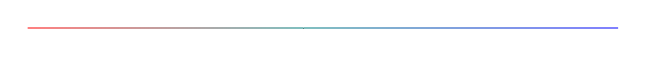
\begin{tikzpicture}
	\fill [left color=red!50, right color=teal!50] (0,0) rectangle (3.5,.01);
	\fill [left color=teal!50, right color=blue!50] (3.5,0) rectangle (7.5,.01);
	\end{tikzpicture}
\vspace{0.5cm}


\vspace{5mm}\begin{large}\textbf{Interpolación de términos en una PA}\end{large}

Interpolar $m$ medios geométricos entre otros dos $a<b$ es encontrar una PG de $m+2$ términos de modo que  $ \ a, \, a_1, \, \cdots ,\,  a_m,\ b$ sea una PG. La razón entre términos será (decimos que son medios porque están entre otros dos y geométricos por tratarse de progresiones geométricas):

$a_n=a_1\,  r^{n-1} \ \to a_{m+2}=\boldsymbol b=a\, r^{(m+2)-1} = 	\boldsymbol{a\, r^{m+1}} \ \to \ \  \boldsymbol{ r=\sqrt[m-1]{\dfrac{b}{a}} }$

\vspace{5mm}

\begin{large} \textbf{Suma de términos consecutivos de una progresión geométrica} \end{large}
\vspace{2mm}

\begin{theorem}

La suma de $n$ términos consecutivos de una PG es:

$$\{a_n\}:\ PG \qquad a_1+a_2+a_3+\cdots + a_{n-1}+a_n= \displaystyle \sum_{k=1}^n	a_k = \ \boxed{ \boldsymbol{S_n\ = \ \ \dfrac{a_n\, r-a_1}{r-1} \ } }$$

\end{theorem}

\underline{Demostración}:

\begin{table}[H]
\centering
\begin{tabular}{lllllll}
$\ S_n \ = \ $ & $a_1$ & $+a_2$  & $+a_3$ & $+ \ \cdots$  & $+a_{n-1}$ & $+a_n$ \\ \hline
$r\cdot S_n=$ & $r\cdot a_1$ & $+r\cdot a_2$  & $+r\cdot a_3$ & $+ \ \cdots$  & $+r\cdot a_{n-1}$ & $+r\cdot a_n$ \\
 & $a_2$ & $+a_3$ & $+a_4$ & $+\ \cdots$ & $+a_n$ & $+r\cdot a_n$ 
\end{tabular}
\end{table}

Restando: $r\cdot S_n-S_n= a_2 +a_3+a_4+\ \cdots+a_n+r\cdot a_n- 
a_1-a_2-a_3- \ \cdots-a_{n-1}-a_n =a_n\, r-a_1$

\vspace{2mm} Despejando: $\quad S_n=\dfrac{a_n\, r-a_1}{r-1}$ \QED

\vspace{0.5cm}

\begin{large} \textbf{Producto de términos consecutivos de una progresión geométrica} \end{large}
\vspace{3mm}

Para ello utilizaremos la siguiente propiedad:

\emph{El producto de términos equidistantes de una PG es igual al producto de sus extremos}, 

$\text{si } a_i,a_j \text{ son términos equidistantes de una PG } \ \Rightarrow \  \boldsymbol{a_i\cdot a_j = a_1\cdot a_n}$


\underline{demostración}: 

$a_i, \, a_j\ $ son términos equidistantes de una PG si $i+j=n+1 \ \to \ j=n+1-i$

$a_i\cdot a_j=a_i\cdot a_{n+1-i}=a_1\, r^{i-1} \cdot a_1\, r^{n+1-i-1}=a_1\ a_1\ r^{i-1\, + \ n+1-i-1}=a_1\, a_1 \, r^{n-1}=a_1\cdot a_n$ \QED

\vspace{0.5cm}

\begin{theorem}

El producto de $n$ términos consecutivos de una PG es:

$$a_1 \cdot a_2 \cdot \cdots \cdot a_n= \displaystyle \prod_{k=1}^n a_k  = \ 
\boxed{ \ \boldsymbol{   
P_n \ = \ \sqrt{ (a_1\cdot a_n)^n } 
} \ }$$	

\end{theorem}

\underline{Demostración}:

\begin{table}[H]
\centering
\begin{tabular}{l|lllll}
$P_n=$ & $a_1\cdot$ & $a_2\cdot$ & $\cdots \cdot$ & $a_{n-1}\cdot$  & $a_n$ \\
$P_n=$ & $a_n\cdot$ & $a_{n-1}\cdot$ & $\cdots \cdot$ & $a_2\cdot$ & $a_1$  \\ \hline
$P_n^2=$ & $(a_1\cdot a_n)$ & $(a_2\cdot a_{n-1})$ & $\cdots$ & $(a_{n-1}\cdot a_2)$  & $(a_n \cdot a_1)$ \\
  & $(a_1\cdot a_n)$  & $(a_1\cdot a_n)$  & $\cdots $  & $(a_1\cdot a_n)$  & $(a_1\cdot a_n)$ 
\end{tabular}
\end{table}

Luego, $\quad P_n^2=(a_1\cdot a_n)^n \quad \to \quad  P_n=\sqrt{(a_1\cdot a_n)^n}$ \QED

\vspace{5mm}

\begin{miejercicio}

Considera la sucesión: $\quad 2,4,8,16,\cdots$

$\quad$ a) Calcula el término general.

$\quad$ b) Calcula la suma de los diez primeros términos.

$\quad$ c) Calcula el producto de los cinco primeros términos.

\rule{250pt}{0.1pt}
\vspace{2mm}

$a)\quad $ Se trata de una $PG \ \begin{cases} \ a_1=2\\\ r=2 \end{cases} \to \ a_n=a_1\cdot r^{n-1}=2\cdot 2^{n-1}=2^n$

\vspace{2mm} $b)\quad a_{10}=2^{10}=1024 \quad \to \quad S_{10}=\dfrac{a_{10}\cdot r-a_1}{r-1}=\dfrac{1024\cdot 2-2}{2-1}=2046$

\vspace{2mm} $c)\quad a_5=2^5=32 \quad \to \quad P_5=\sqrt{(a_1\cdot a_5)^5}=\sqrt{(2\cdot 32)^5}=32768$
	
\end{miejercicio}

\begin{miejercicio}

Interpola 4 medios geométricos entre 1 y 243	.

\rule{250pt}{0.1pt}
\vspace{2mm}

$1, a_1, a_2, a_3, a_4, 243:\ PG \ \quad 243=1\, r^{6-1} \ \Rightarrow \ \  r=\sqrt[5]{\dfrac {243}{1}}=3 \to \, : \quad 1,\ \boldsymbol{3,\, 9,\, 27,\ 81,\ } 243$
\end{miejercicio}



\subsection{Suma de todos los términos de una progresión geométrica}
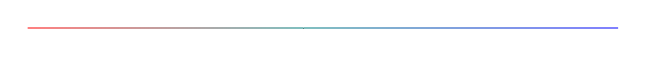
\begin{tikzpicture}
	\fill [left color=red!50, right color=teal!50] (0,0) rectangle (3.5,.01);
	\fill [left color=teal!50, right color=blue!50] (3.5,0) rectangle (7.5,.01);
	\end{tikzpicture}
\vspace{0.5cm}

\begin{theorem}[ Suma de los infinitos términos de una PG]

La suma de todos (infinitos) términos de una PG se puede efectuar siempre que la razón sea, en valor absoluto, menor que la unidad y vale:

$$\boldsymbol{ S_\infty \ = \ \dfrac{a_1}{1-r} } \qquad \qquad \text{siempre que } \ |r|<1$$
	
\end{theorem}


\underline{Demostración}:

Nos basamos en el hecho de que las sucesivas potencias de un número que, en valor absoluto, sea menor que la unidad se acercan cada vez más a cero a medida que aumenta el índice de la potencia, p.e.: $0.1^2=0.01;\ 0.1^{10}=0.0000000001;\ $ etc. Abusando del lenguaje podemos escribir que $r^\infty =0$, siempre que $|r|<1$

Así, $\ \ S_\infty=\dfrac{a_{\infty}r-a_1}{r-1}=\dfrac{a_1\cancelto{0}{r^\infty}-a_1}{r-1}=\dfrac{-a_1}{r-1}=\dfrac{a_1}{1-r}$ \QED

\begin{miejercicio}

Calcula la suma de todos los términos de la sucesión: $\ \dfrac 1 2, \, \dfrac 1 4, \, \dfrac 18, \, \cdots$	


\rule{250pt}{0.1pt}
\vspace{2mm} 

\begin{multicols}{2}
Tenemos una $PG \ \begin{cases} \ a_1=1/2 \\ \ r=1/2 \end{cases}$

$\qquad \text{como } |r|=1/2<1 \quad \to$

$\qquad \to  \quad S_\infty=\dfrac{1/2}{1-1/2}=1$


En la figura siguiente se muestra una \emph{demostración visual}.

\begin{figure}[H]
	\centering
	\includegraphics[width=0.25\textwidth]{img-suc/suc03.png}
\end{figure}
\end{multicols}
\end{miejercicio}
\vspace{1.5cm}%%%%%%%%%%%%%%%%%%%%%%%%%%
\begin{miejercicio}

Lanzamos una pelota a lo largo de un pasillo. En cada bote la pelota avanza una distancia igual a la mitad de la distancia anterior. Si al octavo bote se para, ¿qué distancia ha recorrido si antes del primer bote ha avanzado 2 m? Si no parase de botar, ¿sería necesario un pasillo infinito?

\rule{250pt}{0.1pt}
\vspace{2mm} 

$a_1=2,\, a_2=1,\, a_3=1/2,\, a_4=1/4,\,  \cdots \ :\ \ PG \to a_n=2\, \left(\dfrac 1 2\right)^{n-1}=2^{2-n} \ \Rightarrow \ a_8=\dfrac 1{64}$

\vspace{2mm} $S_8=\dfrac{a_8\cdot r -a_1}{r -1 }=\dfrac{\dfrac 1{64} \, \dfrac 1 2-2 }{1/2-1} \approx 3.98 \,  $m. $\ $ Distancia total recorrida en 8 botes

\vspace{4mm} Salto de $\infty$ botes: $\ \ S_\infty=\dfrac{a_1}{1-r}=\dfrac{2}{1-1/2}=4\, $m. $\ \ $ Distancia total recorrida tras $\infty$ botes, obviamente, no necesitamos un pasillo infinito.

	
\end{miejercicio}

 
\vspace{1.5cm}%%%%%%%%%%%%%%%%%%%%%%%%%%
\begin{figure}[H]
	\centering
	\includegraphics[width=0.95\textwidth]{img-suc/suc09.png}
\end{figure}
\vspace{1.5cm}%%%%%%%%%%%%%%%%%%%%%%%%%%

\vspace{15mm}
\begin{myalertblock}{Progresiones aritmético-geométricas}

\vspace{2mm} Si $a_n$ es una progresión aritmética y $b_n$ es una progresión geométrica, diremos que la sucesión $c_n= a_n \cdot b_n$, de términos $a_1 \cdot b_1,\,  a_2 \cdot  b_2,\,  a_3 \cdot b_3,\, \cdots ,\  $ es una \emph{progresión aritmético-geométrica}.

\vspace{2mm} Está claro que el término general de estas progresiones aritmético-geométricas siempre se puede expresar como  producto de los dos términos generales. Es decir, siempre podremos expresar su término general como $\quad \boldsymbol{c_n=(a\, n+b)\cdot r^n}\, , \quad a\neq 0, \ r\neq 0, \ r\neq 1$


\vspace{2mm} Cálculo de la suma de los $n$ primeros términos:

\vspace{2mm} $S_n=(a+b)r+(2a+b)r^2+(3a+b)r^3+\cdots+(na+b)r^n$

\vspace{2mm} $S_n=ar+2ar^2+3ar^3+\cdots + nar^n\ + \ br+br^2+\cdots br^n$

\vspace{2mm} $rS_n=ar^2+2ar^3+\cdots + nar^{n+1}\ + \ br^2+br^3+\cdot br^{n+1}$

\vspace{2mm} Restando: 

\vspace{2mm} $S_n-rS_n=ar+ar^2+ar^3+\cdots +ar^n-nar^{n+1}+br-br^{n+1}=$

$=ar\left(\dfrac{r^{n-1}\, r-1}{r-1}-nr^n\right)\ + \ br(1-r^n)$

\vspace{2mm} De donde: $\quad \boldsymbol{S_n= \dfrac{
\left( \dfrac{1-r^n}{1-r}-nr^n \right) \ + \ br(1-r^n)
}{1-r}}$

\vspace{2mm} Al igual que con las progresiones geométricas, en estas progresiones se pueden calcular las sumas de los infinitos términos cuando $|r| <1$. En estos casos, teniendo en cuenta que $r^n \approx 0$  cuando $n$ toma valores elevados, tendremos que:

\vspace{2mm}  $\boldsymbol{S_\infty}= \ \dfrac{
\left( \dfrac{1-\cancelto{0}{r^n}}{1-r}-n \cancelto{0}{r^n} \right) \ + \ br(1-\cancelto{0}{r^n})
}{1-r} =\dfrac{ar\left( \dfrac 1{1-r} \right) +br}{1-r} = \ \boldsymbol{\dfrac{ar+br(1-r)}{(1-r)^2}}$
 
 
\vspace{5mm} \underline{Ejemplo}:  calcula la suma de los infinitos términos de la sucesión cuyos primeros términos son de términos $4, 4, 3, 2, 5/4 , \cdots $

\vspace{2mm} Con un poco de astucia se puede ver que: $\ \ 4, 4, 3, 2, 5/4 , \cdots \ = \ \dfrac{8}{2},\, \dfrac{16}{4},\, \dfrac{24}{8},\, \dfrac{32}{16},\, \dfrac{40}{32},\, \cdots$, 

que es una progresión aritmético-geométrica de termino general $\ a_n=\frac{8n}{2^n} \, , \  $ en donde $ a=8;\ b=0;\ r=1/2<1$, por lo que sí se pueden sumar los infinitos términos siendo en resultado de la suma:
$\quad S_\infty= \dfrac{8\cdot 1/2 + 0}{(1-1/2)^2}=\dfrac{4}{1/4}=16$


\end{myalertblock}


\vspace{1cm}
\section{Monotonía y acotación}

\begin{tikzpicture}
	\fill [left color=red!50, right color=teal!50] (0,0) rectangle (3.5,.1);
	\fill [left color=teal!50, right color=blue!50] (3.5,0) rectangle (7.5,.1);
	\end{tikzpicture}
\vspace{0.5cm}


Empecemos con unos ejemplos:

\begin{miejemplo}

\begin{itemize}
\item La sucesión $\ 2,4,8,16,\cdots \ $ es \emph{monótona creciente} (cada término es mayor que el anterior, $\ a_{n+1}>a_n,\ \forall n \in \mathbb N$), pero no está \emph{acotada} (no existe ningún número que no llegue a superar la sucesión $\ \nexists K\in \mathbb R \, / \, a_n<K$).
\item La sucesión $\ 1,-1,1,-1,\cdots \ $no es monótona (ni creciente ni decreciente) pero sí está acotada (p.e. $\ -2<a_n<2\, , \  \forall  n\in \mathbb N \, $)	
\item La sucesión $\ 1,1/2,1/4,1/16,\cdots = 1,0.5,0.25,0.125,\cdots\ $ es monótona decreciente $(a_{n+1}<a_n)$ y está acotada ($\forall n\in \mathbb N\, : \ 0<a_n<2\, $ p.e.)
\end{itemize}
\end{miejemplo}

\begin{definition}[ Monotonía]

\vspace{2mm} Decimos que $a_n$ es \emph{monótona creciente} si $a_{n+1}>a_n,\ \forall n\in \mathbb N$	

\vspace{2mm} Decimos que $a_n$ es \emph{monótona decreciente} si $a_{n+1}<a_n,\ \forall n\in \mathbb N$	

\vspace{4mm} Decimos que $a_n$ es \emph{monótona} si lo es de modo creciente o decreciente.

\vspace{4mm} Si $a_n$ crece y decrece alternativamente en términos sucesivos, se la llama sucesión \emph{oscilante}.
\end{definition}

\begin{definition}[ Acotación]

\vspace{2mm} Decimos que $a_n$ está \emph{acotada superiormente} si $\ \exists K\in \mathbb R ,\ / \, a_n<K ,\ \forall n\in \mathbb N\ $ ($K$ cota superior)	 

\vspace{2mm} Decimos que $a_n$ está \emph{acotada inferiormente} si $\ \exists M\in \mathbb R ,\ / \, a_n>M ,\ \forall n\in \mathbb N\ $	 ($M$ cota inferior)
	

\vspace{4mm} Decimos que $a_n$ está \emph{acotada} si lo está de superior e inferiormente, 

\textcolor{gris}{si $\ \exists L\in \mathbb R \, / \, |a_n|<L,\ \forall n\in \mathbb N\ $} ($L$ cota)
\end{definition}

\vspace{5mm}
\begin{miejercicio}

Da un ejemplo de 

\begin{enumerate}[a) ]	
\vspace{-2mm} \item Sucesión decreciente y no acotada.
\vspace{-2mm} \item Sucesión creciente y acotada.
\vspace{-2mm} \item	Sucesión no monótona y no acotada.
\end{enumerate}

\rule{250pt}{0.1pt}
\vspace{2mm}
\begin{enumerate}[a) ]	
\item $\quad -1,-10,-100,-1000,\cdots$
\item $\quad 1,1.1,1.11,1.111,\cdots \quad$ \textcolor{gris}{(pe, 2 es una cota)}
\item $\quad 1,-2,3,-4,\cdots $
\end{enumerate}

\end{miejercicio}


\vspace{1cm}
\section{Idea intuitiva de límite de una sucesión}

\begin{tikzpicture}
	\fill [left color=red!50, right color=teal!50] (0,0) rectangle (3.5,.1);
	\fill [left color=teal!50, right color=blue!50] (3.5,0) rectangle (7.5,.1);
	\end{tikzpicture}
\vspace{0.5cm}

\begin{definition} [ Convergencia]

\begin{itemize}
\item Llamamos \emph{límite} de una sucesión $a_n$ a un número $L \in \mathbb R$, si existe, al cual se acercan progresivamente los términos de la sucesión a medida que $n$ toma valores más grandes. Lo representamos por  $\underset{n\to \infty}{\mathrm{lim}} a_n=L$ y decimos	 que $a_n$ es una sucesión \emph{convergente} ($a_n$ converge a $L$).

Si una sucesión no es convergente se dice que es \emph{divergente}

\item Si la sucesión va tomando valores cada vez mayores a medida que $n$ aumenta, superando a cualquier número real $K\in \mathbb R$, decimos que $a_n$ es \emph{divergente} a $+\infty$ y lo representamos como $\underset{n\to \infty}{\mathrm{lim}} a_n=+\infty$ ($a_m$ diverge a $+\infty$).
\item Si ocurre lo mismo para números negativos, siempre se pueden encontrar términos de la sucesión menores que cualquier  número real $K\in \mathbb R$, decimos que la sucesión es divergente a $-\infty$ y lo representamos por $\underset{n\to \infty}{\mathrm{lim}} a_n=-\infty$
\end{itemize}
	
\end{definition}

\begin{miejercicio}

Da un ejemplo de:

\begin{enumerate}[a) ]	
\vspace{-2mm} \item Sucesión oscilante y convergente.
\vspace{-2mm} \item Sucesión oscilante, no acotada y divergente.
\vspace{-2mm} \item	Sucesión oscilante, acotada y divergente.

\vspace{-2mm} \item Sucesión creciente y acotada (convergente).
\vspace{-2mm} \item Sucesión decreciente y acotada (convergente).
\vspace{-2mm} \item Sucesión creciente y no acotada (divergente).
\end{enumerate}

\rule{250pt}{0.1pt}

\begin{enumerate}[a) ]	
\item $5.1,\ 4.9,\ 5.01, 4.99,\ 5.001,\ 4.999,\ \cdots \qquad  \qquad \textcolor{gris}{\underset{n\to \infty}{\mathrm{lim}} a_n=5}$
\item $1,\ -10, \ 100,\ -1000, \ \cdots \qquad  \qquad \textcolor{gris}{\nexists \underset{n\to \infty}{\mathrm{lim}} b_n}$
\item $5,\ -5,\ 5,\ -5,\ \cdots \qquad  \qquad \textcolor{gris}{\nexists \underset{n\to \infty}{\mathrm{lim}} c_n}$
\item $8,\ 8.9,\ 8.99,\ 8.999,\ \cdots \qquad  \qquad \textcolor{gris}{\underset{n\to \infty}{\mathrm{lim}} d_n=9}$
\item $9.1,\ 9.01,\ 9.001,\ 9.0001,\ \cdots \qquad  \qquad \textcolor{gris}{\underset{n\to \infty}{\mathrm{lim}} e_n=9}$
\item $1,2,3,4,\cdots \qquad  \qquad \textcolor{gris}{\underset{n\to \infty}{\mathrm{lim}} f_n=+\infty}$ 
\end{enumerate}
	
\end{miejercicio}

\vspace{1cm}

\begin{myexampleblock}{El número e}

El número $ \boldsymbol e \, , \  $ (número de Euler o constante de Napier) base de los logaritmos naturales,  se define como el límite de una sucesión: 

$$\boldsymbol{ e=\underset{n\to \infty}{\mathrm{lim}} \left( 1+\dfrac 1 n \right)^n}$$

\vspace{2mm} Para $n=100 \to e=2.7;\quad n=1000\to e=2.71;\quad n=10^6 \to e=2.71828$. El número $e$ es un número irracional, con infinitas cifras decimales no periódicas (como $\pi$).

\vspace{2mm} Desarrollando el binomio de Newton:

\vspace{2mm} $\left( 1+\dfrac 1 n \right)^n=1+n\dfrac 1 n + \mqty(n\\2) \left( \dfrac 1 n \right)^2+\mqty(n\\3) \left( \dfrac 1 n \right)^3+ \cdots + \mqty(n\\n) \left( \dfrac 1 n \right)^n=1+1+\dfrac {1}{2!} \dfrac{n(n-1)}{n^2}+ \dfrac {1}{3!} \dfrac{n(n-1)(n-2)}{n^3}+ \cdots = 1+1\dfrac{1}{1!} +\dfrac{1}{2!} \left(1-\dfrac 1 n \right)+\dfrac{1}{3!} \left(1-\dfrac 1 n \right)\left(1-\dfrac 2 n \right)+\cdots$

\vspace{2mm} Teniendo en cuenta que $\dfrac 1 n \approx 0$ cuando $n \to \infty$ y tomando límites en la expresión anterior:

$$\boldsymbol{e} \ =\underset{n\to \infty}{\mathrm{lim}} \left( 1+\dfrac 1 n \right)^n \ = \ 1+\dfrac {1}{1!} + +\dfrac {1}{2!} +\dfrac {1}{3!} + \cdots +\dfrac {1}{n!} + \cdots = \ \boldsymbol{\sum_{n=0}^\infty \dfrac {1}{n!}}$$ 

\vspace{2mm} $e$ también puede expresarse como la suma de una sucesión. De este modo se obtienen aproximaciones  del número $e$ mucho más rápidamente, basta con tomar $8$ términos para conseguir $5$ decimales (antes necesitábamos tomar $n=1000000$): $\ e\approx 2.71828\cdots$

\vspace{2mm} 
	
\end{myexampleblock}



\vspace{1cm}
\section{Ejercicios}

\begin{tikzpicture}
	\fill [left color=red!50, right color=teal!50] (0,0) rectangle (3.5,.1);
	\fill [left color=teal!50, right color=blue!50] (3.5,0) rectangle (7.5,.1);
	\end{tikzpicture}
\vspace{0.5cm}

%************
\begin{mipropuesto}

Encuentra el término general de las siguientes sucesiones:

\begin{multicols}{3}
\begin{enumerate}[a) ]
\item $\ \dfrac{1}{2},\dfrac{2}{3},\dfrac{3}{4},\dfrac{4}{5},\dfrac{5}{6},\cdots$
\item $\ \dfrac{1}{2},\dfrac{1}{3},\dfrac{1}{4},\dfrac{1}{5},\cdots$
\item $\ \dfrac{1}{5},\dfrac{4}{7},\dfrac{9}{9},\dfrac{16}{11},\dfrac{25}{13},\cdots$
\item $\ 0,\dfrac{3}{5},\dfrac{8}{10},\dfrac{15}{17},\dfrac{24}{26},\cdots$
\item $2,5,10,17,26,\cdots$
\item $7,-7,7,-7,7,\cdots$

\end{enumerate}
	
\end{multicols}

\end{mipropuesto}

\vspace{-8mm}
\begin{flushright}
	\begin{footnotesize} \textcolor{gris}{\rotatebox{180}{ $a_n=\frac{n}{n+1};\quad b_n=\dfrac{1}{n+1};\quad c_n=\dfrac{n^2}{2n+3};\quad d_n=\dfrac{n^2-1}{n^2+1};\quad e_n=n^2+1;\quad f_n=(-1)^{n+1}\cdot 7$ }}	\end{footnotesize}
	
	\begin{footnotesize} \textcolor{gris}{\rotatebox{180}{ Busca el término general del numerador y denominador por separado. }}	\end{footnotesize}
\end{flushright}







%************
\begin{mipropuesto}

Encuentra el término general de las siguientes sucesiones:
\begin{multicols}{2}
\begin{enumerate}[a) ]
\item $1.2,\, 2.4,\, 3.6,\, 4.8,\, 6,\, \cdots$
\item $1,\, 0.1,\ 0.01,\, 0.001,\ 0.0001,\, \cdots$
\item $1, \, \dfrac{89}{100}, \, \dfrac{78}{100}, \, \dfrac{67}{100}, \, \dfrac{56}{100},\, \cdots$
\item $\sqrt{2}, \, 2,\, 2\sqrt{2},\, 4,\, 4\sqrt{2},\, \cdots$
\end{enumerate}
	
\end{multicols}

\end{mipropuesto}

\vspace{-8mm}
\begin{flushright}
\begin{footnotesize} \textcolor{gris}{\rotatebox{180}{ $a_n=1.2n;\quad b_n=0.1^{n-1};\quad c_n=\dfrac{111-11n}{100};\quad d_n=(\sqrt{2})^n$ }}	\end{footnotesize}
\end{flushright}




%************
\begin{mipropuesto}

En una progresión aritmética sabemos que $a_2= 1$ y $a_5=7$. Halla el término general y calcula la suma de los $15$ primeros términos.
\end{mipropuesto}

\vspace{-8mm}
\begin{flushright}
\begin{footnotesize} \textcolor{gris}{\rotatebox{180}{ Puedes plantear un sistema para encontrar $a_1$ y $d$. $\quad a_n=2n-3 ;\quad S_{15}=195 $ }}	\end{footnotesize}
\end{flushright}


%************
\begin{mipropuesto}

En una progresión geométrica sabemos que $a_1= 3$ y $a_4=24$. Halla la razón y calcula la suma de los $8$ primeros términos.
\end{mipropuesto}

\vspace{-8mm}
\begin{flushright}
\begin{footnotesize} \textcolor{gris}{\rotatebox{180}{ $r=2 ;\quad S_{15}=765 $ }}	\end{footnotesize}
\end{flushright}



%************
\begin{mipropuesto}

Los ángulos de un triángulo están en progresión aritmética. Sabiendo que el mayor de ellos mide $105^o$, ?`cuánto miden los otros dos?
\end{mipropuesto}

\vspace{-8mm}
\begin{flushright}
\begin{footnotesize} \textcolor{gris}{\rotatebox{180}{ Ayuda: la suma de los ángulos de un triángulo suman $180^o\qquad $ Sol.: $15^o \text{ y } 60^o$  }}	\end{footnotesize}
\end{flushright}



%**********
\begin{mipropuesto}

En una urbanización realizaron la instalación del gas natural en el año 1999. Consideramos que en ese momento se hizo la primera revisión.

\vspace{2mm} Sabiendo que las revisiones sucesivas se realizan cada 3 años, responde:

\vspace{2mm} a) ?`En qué año se realizará la décima revisión?

b) ?`Cuál es el número de revisión que se realizará en el año 2035?

c) ?`Se realizará revisión en el 2022?
\end{mipropuesto}

\vspace{-8mm}
\begin{flushright}
\begin{footnotesize} \textcolor{gris}{\rotatebox{180}{ PA:$\quad a)\ 2026;\quad b)\ 13;\quad c)\ \text{No}$ }}	\end{footnotesize}
\end{flushright}




%************
\begin{mipropuesto}

La población de un cierto país aumenta por término medio un 1\% anual. Sabiendo que en la actualidad tiene 3 millones de habitantes:
a) ?`Cuántos tendrá dentro de 10 años?;  b) ?`Y dentro de 20 años?
\end{mipropuesto}

\vspace{-8mm}
\begin{flushright}
\begin{footnotesize} \textcolor{gris}{\rotatebox{180}{ PG: $\qquad a)\ 3313866;\quad b)\ 3660570$ }}	\end{footnotesize}
\end{flushright}



%**********
\begin{mipropuesto}

Una máquina costó inicialmente 10480 \euro. Al cabo de unos años se vendió a la mitad de su precio. Pasados unos años, volvió a venderse por la mitad, y así sucesivamente.

\vspace{2mm} a) ?`Cuánto le costó la máquina al quinto propietario?

b) Si el total de propietarios ha sido 7, ?`cuál es la suma total pagada por esa máquina?
\end{mipropuesto}

\vspace{-8mm}
\begin{flushright}
\begin{footnotesize} \textcolor{gris}{\rotatebox{180}{ PG: $\qquad a)\ 655 $ \euro; $\quad b)\ 163.75 $ \euro }}	\end{footnotesize}
\end{flushright}



%************
\begin{mipropuesto}

Calcula la suma de todos los números impares de tres cifras.
\end{mipropuesto}

\vspace{-8mm}
\begin{flushright}
\begin{footnotesize} \textcolor{gris}{\rotatebox{180}{ $247500$ }}	\end{footnotesize}
\end{flushright}



%**********
\begin{mipropuesto}

En un cine, la segunda fila de butacas está a 10 m de la pantalla y la séptima fila está a 16 m. ?`En qué fila debe sentarse una persona que le guste ver la pantalla a una distancia de 28 m?
\end{mipropuesto}

\vspace{-8mm}
\begin{flushright}
\begin{footnotesize} \textcolor{gris}{\rotatebox{180}{ Fila 17 }}	\end{footnotesize}
\end{flushright}



%************
\begin{mipropuesto}

La sucesión 1, 1, 1, 1, ... puede considerarse una progresión aritmética y también geométrica. ?`Cuál es la diferencia en el primer caso? ?`Y la razón en el segundo?

\end{mipropuesto}

\vspace{-8mm}
\begin{flushright}
\begin{footnotesize} \textcolor{gris}{\rotatebox{180}{ $d=0;\ \ \ r=1$ }}	\end{footnotesize}
\end{flushright}



%**********
\begin{mipropuesto}

Dados estos dos términos de una sucesión, $a_1 = 2$ y $a_3 = 8$, halla cuatro términos más y el término
general suponiendo que se trata de una progresión: a) aritmética; b) geométrica.
\end{mipropuesto}

\vspace{-8mm}
\begin{flushright}
\begin{footnotesize} \textcolor{gris}{\rotatebox{180}{ $a_2,a_4,a_5,a_6,\ a_n: \qquad a)\ PA:\ 5,11,14,17, \ 3n-1;\qquad b)\ PG:\ 4,16,32,62,\ 2^n$ }}	\end{footnotesize}
\end{flushright}



%************
\begin{mipropuesto}

La dosis de un medicamento es 100 mg el primer día y 5 mg menos cada uno de los siguientes. El tratamiento dura 12 días. ?`Cuántos miligramos tiene que tomar el enfermo durante todo el tratamiento?
\end{mipropuesto}

\vspace{-8mm}
\begin{flushright}
\begin{footnotesize} \textcolor{gris}{\rotatebox{180}{ $870$ mg }}	\end{footnotesize}
\end{flushright}



%**********
\begin{mipropuesto}

Un tipo de bacteria se reproduce por bipartición cada cuarto de hora. ?`Cuántas bacterias habrá después de 6 horas?

\end{mipropuesto}

\vspace{-8mm}
\begin{flushright}
\begin{footnotesize} \textcolor{gris}{\rotatebox{180}{ $8 388 608$ }}	\end{footnotesize}
\end{flushright}


%************
\begin{mipropuesto}

\begin{figure}[H]
	\centering
	\includegraphics[width=0.75\textwidth]{img-suc/suc07.png}
\end{figure}


\end{mipropuesto}

\vspace{-8mm}
\begin{flushright}
\begin{footnotesize} \textcolor{gris}{\rotatebox{180}{ Nums. cuadrangulares: $\quad 1^2,\ 2^2,\ 3^2,\ 4^2,\ \cdots \ \to \ C_n=n^2$ }}	\end{footnotesize}
\end{flushright}
\vspace{-10mm}
\begin{flushright}
\begin{footnotesize} \textcolor{gris}{\rotatebox{180}{ Nums. triangulares. $\quad 1,\ 1+2,\ 1+2+3,\ 1+2+3+4,\ \cdots \ \to \ T_n=n(n+1)/2$ }}	\end{footnotesize}
\end{flushright}


%************
\begin{mipropuesto}

\begin{multicols}{2}

De la siguiente sucesión de cuadrados, calcula:

\vspace{3mm} a) Sucesión que define las áreas de cada cuadrado.	

b) Sucesión de las longitudes de sus lados.

c) Suma de las áreas de todos ellos.

\begin{figure}[H]
	\centering
	\includegraphics[width=0.35\textwidth]{img-suc/suc04.png}
\end{figure}


\end{multicols}

\end{mipropuesto}

\vspace{-8mm}
\begin{flushright}
\begin{footnotesize} \textcolor{gris}{\rotatebox{180}{ $a_n=2^{7-n};\qquad b_n=2^{\frac{7-n}{2}} \, \mathrm{cm} ;\qquad S_\infty=128 \, \mathrm{cm}^2$ }}	\end{footnotesize}
\end{flushright}



%**********
\begin{mipropuesto}

\begin{multicols}{2}

Considera un triángulo equilátero de 16 cm de lado. Se unen los puntos medios de sus lados para obtener 4 nuevos triángulo más pequeños. En estos triángulos se vuelven a unir los puntos medios, y así sucesivamente. Calcula:

a) Sucesión que define el área de los triángulos obtenidos.	

b) Sucesión de las longitudes de sus lados.

c) Sucesión de las áreas de todos ellos.

\begin{figure}[H]
	\centering
	\includegraphics[width=0.4\textwidth]{img-suc/suc05.png}
\end{figure}


\end{multicols}

\end{mipropuesto}

\vspace{-8mm}
\begin{flushright}
\begin{footnotesize} \textcolor{gris}{\rotatebox{180}{ $a_n=4^{n-1};\qquad l_n=2^{5-n};\qquad a_n=2^{8-2n}\sqrt{3}$ }}	\end{footnotesize}
\end{flushright}

%********

\begin{mipropuesto}

Interpola 6 términos entre 1 y 10 que formen una PA.
\end{mipropuesto}

\vspace{-8mm}
\begin{flushright}
\begin{footnotesize} \textcolor{gris}{\rotatebox{180}{ $16/7,\ 25/7,\ 34/7,\ 43/7,\ 52/7,\ 61/7$ }}	\end{footnotesize}
\end{flushright}


%********

\begin{mipropuesto}

Interpola tres términos entre 1 y 16 para que formen una PG.
\end{mipropuesto}

\vspace{-8mm}
\begin{flushright}
\begin{footnotesize} \textcolor{gris}{\rotatebox{180}{ $r^4=16 \to |r|=2 \to r=\pm 2:\ \ \text{ Sol.: }\  \pm 2,\ 4,\ \pm 8$ }}	\end{footnotesize}
\end{flushright}



%********

\begin{mipropuesto}

En un examen la primera pregunta vale 2 puntos y cada una de las siguientes vale 3 puntos más que la anterior. Si en total hay 50 preguntas, ?`cuántos puntos vale el examen?
\end{mipropuesto}

\vspace{-8mm}
\begin{flushright}
\begin{footnotesize} \textcolor{gris}{\rotatebox{180}{ PA: 3775 }}	\end{footnotesize}
\end{flushright}



%********

\begin{mipropuesto}

Inicialmente hay 50 moscas en un laboratorio y, cada tres días, el número de moscas se duplica. ?`Cuántas moscas habrá al cabo de un mes?
\end{mipropuesto}

\vspace{-8mm}
\begin{flushright}
\begin{footnotesize} \textcolor{gris}{\rotatebox{180}{ PG (1mes=30 días). Habrá 16000 moscas. }}	\end{footnotesize}
\end{flushright}



%********

\begin{mipropuesto}

Los ángulos de un triángulo están en PA, si el ángulo intermedio vale $60^o$, ?`qué puedes afirmar de la distancia de la progresión?
\end{mipropuesto}

\vspace{-8mm}
\begin{flushright}
\begin{footnotesize} \textcolor{gris}{\rotatebox{180}{ (Dos ángulos han de sumar menos de $180^o$) $\quad$ $-60<d<60$ }}	\end{footnotesize}
\end{flushright}




%%%%%%%%%%%%%%%%%%%%%%%%%%%%.  problemas +.   %%%%%%%%%%%%%%%%%%%%
\newpage
\begin{adjustwidth}{50pt}{250pt}
\begin{cuadro-naranja}
\textbf{\huge{Problemas $\boldsymbol{+}$}}\normalsize{$\, $}
\end{cuadro-naranja}	
\end{adjustwidth}

\vspace{5mm}
\begin{enumerate}[\textbf{P$\boldsymbol +$} 1. ]

%
\item	Demostrar que las sucesivas medias de $n$ primeros términos de una progresión aritmética de distancia $d$ forman una progresión aritmética de distancia $d/2$.

\vspace{-6mm}
\begin{flushright}
\begin{footnotesize} \textcolor{gris}{\rotatebox{180}{ $x_n:\ PA[x_1,d/2]\, \  \text{ hay que demostrar que  } \ x_{n+1}-x_n=d/2$ }}

 \textcolor{gris}{\rotatebox{180}{ $a_n:\ PA[a_1,d]\qquad x_1=a_1,\ x_2=(a_1+a_2)/2,\ x_3=(a_1+a_2+a_3)/3,\ \cdots$ }}	\end{footnotesize}
\end{flushright}


%
\item	La suma de 18 números naturales consecutivos es un cuadrado perfecto, ?`cuál es el menor valor posible de la suma de ellos?

\vspace{-6mm}
\begin{flushright}
\begin{footnotesize} \textcolor{gris}{\rotatebox{180}{ $PA[a_1,\, d=1]\to \text{ cuadrado perfecto mínimo si  } a_1=4 \ \to \ S_{18}=15^2$ }}	\end{footnotesize}
\end{flushright}


%
\item	Si $a_n$ es PA y también PG y sabemos que $a_1=5$, ?`qué vale $a_5$? 

\vspace{-6mm}
\begin{flushright}
\begin{footnotesize} \textcolor{gris}{\rotatebox{180}{ $5$ en ambos casos. }}	\end{footnotesize}
\end{flushright}


%
\item	Fíjate en la siguiente figura, ?`puedes generalizar el resultado?

\begin{figure}[H]
	\centering
	\includegraphics[width=0.5\textwidth]{img-suc/suc06.png}
\end{figure} 

\vspace{-10mm} %%%%%
\begin{flushright}
\begin{footnotesize} \textcolor{gris}{\rotatebox{180}{ Piensa en lo que ocurre a partir de la posición segunda.  $\quad a_1=1,\ \ a_n=n^2-n-1,\ \forall n\geq 2$}}	\end{footnotesize}
\end{flushright}


%
\item	Los primeros términos de una PG son: $ \ \sqrt{2}+1,\, 1,\ \sqrt{2}-1,\ \cdots $
La suma de \emph{todos} sus términos puede expresarse como $\ S_\infty=\dfrac{a+b\sqrt{c}}{d}.\ $ ?`Cuál es el valor mínimo de $a+b+c+d$? 

\vspace{-6mm}
\begin{flushright}
\begin{footnotesize} \textcolor{gris}{\rotatebox{180}{ $s_\infty=\frac{4+3\sqrt{2}}{2} \ \to \ a+b+c+d=11,\ $ valor mínimo pues expresión está simplificada al máximo. }}	\end{footnotesize}
\end{flushright}


%
\item	Si $f_n$ designa el término $n$-simo de la sucesión de Fibonacci \textcolor{gris}{$[ \ f_1=1,\ f_2=1,\ f_n=f_{n-1}+f_{n-2},\, \forall n>2 \ ]$} y conociendo que $f_{28}=317811$ y que $f_{24}=46368$, usando estos datos, determina el valor de $f_{26}$.

\vspace{-6mm}
\begin{flushright}
\begin{footnotesize} \textcolor{gris}{\rotatebox{180}{ Escribe $f_{26}$ en función de $f_{24}$ y $f_{28}$ usando la recurrencia de la sucesión. $\quad$ $f_{26}=121393$  }}	\end{footnotesize}
\end{flushright}


%
\item	En la sucesión $ \ a_1,a_2,a_3,\cdots \ $ se cumple que $a_1=a,\  a_3=b,\ a_{n+1}=a-n+a_{n+2}-1,\, \forall n\geq 2. \ $ Calcula la suma de los $2022$ primeros términos.

\vspace{-4mm}
\begin{flushright}
\begin{footnotesize} \textcolor{gris}{\rotatebox{180}{y, a partir de ahí, la sucesión se repite. Como $2022=337\times 6 \to S_{2020}=337\times 6$ }}	\end{footnotesize}

\begin{footnotesize} \textcolor{gris}{\rotatebox{180}{ Busca los primeros términos de la sucesión hasta que caigas en la cuenta de que $a_1+\cdots +a_6=6$  }}	\end{footnotesize}
\end{flushright}

%
\item	Dados los tres primeros términos de una PG: $\ \sqrt{7},\ \sqrt[3]{7},\ \sqrt[6]{7}\, , \ $ ?`cuál es el siguiente término de la progresión?

\vspace{-6mm}
\begin{flushright}
\begin{footnotesize} \textcolor{gris}{\rotatebox{180}{ 1 }}	\end{footnotesize}
\end{flushright}

%
\item	Los números $\ \log(a^3b^7),\ \log(a^5b^{12}),\ \log(a^8b^{15})\ $ son los tres primeros términos de una PA en la que $\ \log(b^n)\ $ es el duodécimo termino. ?`Qué vale $n$?

\vspace{-6mm}
\begin{flushright}
\begin{footnotesize} \textcolor{gris}{\rotatebox{180}{ 112 }}	\end{footnotesize}
\end{flushright}

%
\item	En una PA de 9 términos el quinto es 4. ?`Cuánto suman los 9 términos?

\vspace{-6mm}
\begin{flushright}
\begin{footnotesize} \textcolor{gris}{\rotatebox{180}{ Equidistancia, $a_5$ es el término central. $\quad$ sol: $\ 36$ }}	\end{footnotesize}
\end{flushright}


\end{enumerate}



%%%%%%%%%%%%%%%%%%%%%%%%%%%%%%%%%%%%
\newpage
\section{Resumen del tema}

\begin{tikzpicture}
	\fill [left color=red!50, right color=teal!50] (0,0) rectangle (3.5,.1);
	\fill [left color=teal!50, right color=blue!50] (3.5,0) rectangle (7.5,.1);
	\end{tikzpicture}
\vspace{1cm}

\begin{myblock}{Resumen: \emph{``Sucesiones''}}

\vspace{2mm}\textbf{Progresión aritmética}: cada término se obtiene del anterior al sumar una cantidad constante llamada distancia.

$$\boxed{ \ \boldsymbol{a_n\ = \ a_1\, + \, (n-1)\, d}  \ } 
\qquad \qquad
 \boxed{\ \boldsymbol{ S_n\ = \ \dfrac{a_1+a_n}{2}\ n } \ }$$
 
\vspace{5mm} \textbf{Progresión geométrica}: cada término se obtiene del anterior al multiplicar una cantidad constante llamada razón.

$$\boxed{\ \boldsymbol{ a_n\ = \ a_1\, r^{n-1} } \ }
\qquad \qquad	
\boxed{\ \boldsymbol{ S_n\ = \ \dfrac{a_n\, r - a_1}{r-1} } \ }$$

$$\boxed{\ \boldsymbol{ S_\infty \ = \ \dfrac{a_1}{1-r}  } \ } \ \ \leftrightarrow \ \ |r|<1
\qquad \qquad	
\boxed{\ \boldsymbol{ P_n\ = \ \sqrt{(a_1\, a_n)^n} } \ }$$

\vspace{5mm} \textbf{Interpolar} $m$ medios (aritméticos o geométricos) entre dos números dados $a$ y $b$ es encontrar $m$ números $a_1,a_2,\cdots , a_m$ de modo que la sucesión $a,a_1,a_2,\cdots , a_m,b$ formen una progresión (aritmética o geométrica).

\vspace{5mm}$\triangleright \quad   \{a_n\} \ $ es una sucesión \textbf{monótona creciente } si $\ a_{n+1}>a_n\, , \ \ \forall n\in \mathbb N$


\vspace{2mm}$\triangleright \quad \{a_n\} \ $ es una sucesión \textbf{monótona decreciente } si $\ a_{n+1}<a_n\, , \ \ \forall n\in \mathbb N$

\vspace{5mm}$\triangleright \quad \{a_n\} \ $ es una sucesión\textbf{ acotada } si $\ \exists K \in \mathbb R \, / \,  |a_n|\leq K , \ \ \forall n\in \mathbb N$

\vspace{5mm}$\triangleright \quad \{a_n\} \ $ es una sucesión\textbf{ convergente  } si $\ \exists \ \underset{n\to \infty}{\mathrm{lim}}\, a_n$

\vspace{2mm}

\end{myblock}

















\begin{comment}


%%%%%%%%%%%%%%% EJER PPTO
Un atleta quiera preparar una carrera y entrenará, de forma constante, el número de metros que corre cada día. Cada día correrá una cantidad de metros constante más que el día anterior.

Empieza a correr el lunes 280 m y quiere llegar a correr el domingo 1km. ?`Cuánto debe correr cada día.
%%%%%%%%%%%%%%%%%%%%%




%%%%%%%%%%%%%%%%%%%%%%%%%%%%%%%%%%%. SECCIONES
\chapter{texto}

\begin{tikzpicture}
	\fill [left color=red!50, right color=teal!50] (0,0) rectangle (6.5,.2);
	\fill [left color=teal!50, right color=blue!50] (6.5,0) rectangle (11.5,.2);
	\end{tikzpicture}

\vspace{1cm}
\section{texto}

\begin{tikzpicture}
	\fill [left color=red!50, right color=teal!50] (0,0) rectangle (3.5,.1);
	\fill [left color=teal!50, right color=blue!50] (3.5,0) rectangle (7.5,.1);
	\end{tikzpicture}
\vspace{0.5cm}

\subsection{texto}
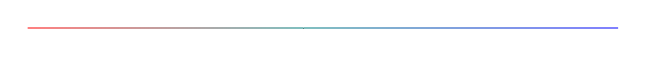
\begin{tikzpicture}
	\fill [left color=red!50, right color=teal!50] (0,0) rectangle (3.5,.01);
	\fill [left color=teal!50, right color=blue!50] (3.5,0) rectangle (7.5,.01);
	\end{tikzpicture}
\vspace{0.5cm}


%%%%%%%%%%%%%%%%%%%%%%%%%%%%%%%%%%%. \begin{ ------>. 
detsacado;  cuadro-naranja;  cuadro-gris;  miejercicio (solución extensa);  mipropuesto (solución corta y fuera del cuadro)

%%%%%%%%%%%%%%%%%%%%%%%%%%%%%%%%%%%. CURIOSIDAD
\vspace{1cm}
\color{ForestGreen!80}
\rule{250pt}{0.2pt}
Texto
\vspace{-8mm}
\begin{flushright}
\rule{250pt}{0.2pt}		
\end{flushright}	
\color{black}




IMAGENES%******************************
\begin{figure}[H]
	\centering
	\includegraphics[width=0.75\textwidth]{img-reales/reales18.png}
	\end{figure}
\end{comment}